\chapter{Experimental Methodology}
\label{methodology}

\section{Anechoic Chamber}
All experiments were conducted at the GDTL within the Aerospace Research Center at the Ohio State University. 
Compressed, dried, and filtered air is supplied to the facility from two cylindrical storage tanks with a total capacity of 43 m$^{3}$ and maximum storage pressure of 16 MPa.
The air may be routed through a storage heater, which allows the jet to operate with a stagnation temperature up to 500~$^\circ$C, before expanding through a nozzle and exhausting horizontally into an anechoic chamber. 
As the current work was focused on a cold jet, the heater was rarely necessary; in certain circumstances though (namely, long experimental runs) the storage heater and bandheaters were used to slightly preheat the flow, thereby mitigating the temperature drop as the storage tanks were drained of high-pressure air.
Opposite the nozzle, a collector accumulates the jet and exhausts to the outdoors. 
A schematic of the anechoic chamber can be seen in \fig{fig:chamber}. 
The dimensions of the chamber are 6.20 m wide by 5.59 m long and 3.36 m tall, with internal wedge-tip to wedge-tip dimensions of 5.14 m by 4.48 m and 2.53 m, respectively. 
The design of the chamber produces a cutoff frequency of 160 Hz, below the frequencies of interest for this study. 
A more detailed description of the GDTL anechoic chamber properties and validation has been given by Hahn \citep{Hahn2011}.
\begin{figure}
	\centering
	\includegraphics{Figures/Chamber_Schematic.png}
	\caption{Top-down view of anechoic chamber and free jet facility at GDTL; dimensions are in meters.} 
	\label{fig:chamber}
\end{figure}

For this study a converging, axisymmetric nozzle with exit diameter D of 25.4 mm was used. 
The internal contour of the nozzle was designed using a fifth order polynomial. 
The nozzle utilized a thick-lipped design in order to simplify the mounts for the LAFPA extension, which housed the eight actuators used in this study. 
For the experiments reported in this paper, the jet was operated at a Mach number ($M_j$) of 0.90, and with a total temperature ratio of approximately unity. 
The Reynolds number based on the jet exit diameter was $6.2\times〖10〗^5$; previous investigations using hot-wire anemometry have indicated that the initial shear layer is turbulent for this operating condition with momentum thickness ~0.09 mm and boundary layer thickness ~1 mm \citep{Kearney-Fischer2009}.

\section{Localized Arc-Filament Plasma Actuators}
The design of the localized arc-filament plasma actuators, as well as the driving circuitry, has undergone a slow evolution since their initial development by the GDTL and NETL.
In the current work, each LAFPA actuator consists of a pair of 1~mm diameter tungsten pin electrodes.
The center-to-center spacing between electrode pairs for each actuator is 4 mm.
Eight actuators were uniformly spaced around the nozzle perimeter 1 mm upstream of the nozzle exit. 
For electrical and thermal durability, the electrodes were housed in a boron nitride (grade AX05) extension attached to the end of the nozzle. 
A groove with dimensions of 1 mm wide and 0.5 mm deep is machined in the boron nitride, into which the electrode tips protrude, to provide a region of low momentum flow in order to stabilize the plasma arcs. 
It has been shown that the existence of this groove does not substantially alter the flow field or the control authority of the LAFPAs \citep{Hahn2011a}. 
A detailed description of initial development and LAFPA characteristics can be found in Utkin \etal \citep{Utkin2007}.

The LAFPAs were energized by a multi-channel, high-voltage plasma power generator capable of simultaneously powering up to eight LAFPAs, which was designed and built in-house at the GDTL. 
In this second-generation power supply, each individual circuit consists of a switchable capacitor in line with a high voltage transformer; the arcing electrodes are connected to the secondary side of the coil. 
The capacitor is charged by a 100 V DC power supply when the first switch is closed and the second is opened; at the user-specified time the switches flip and it discharges through the coil. 
The switches are controlled by a 16-channel digital I/O card and National Instruments' Labview software, operated by a dedicated computer. The plasma generator provides independent control of the frequency, duty cycle/pulse width, and phase of each individual actuator (though not the amplitude). 
The pulse width was held constant at 7 μs, which was found to be the minimum pulse width at which the actuators consistently arced for all frequencies explored in this study [citation]. 
The circuit is limited to 20 kHz due to thermal concerns.
However, as the current work is focused on the evolution of large-scale structures (and ultimately their acoustic radiation), for which the dominant frequencies are on the order of 3~kHz, this is not an issue.

\section{Data Acquisition}
\subsection{Near- and Far-field Pressure}
Near-field and far-field pressure measurements were acquired using Br\"{u}el \& Kj\ae{}r 0.25-inch 4939 microphones and preamplifiers. 
The signal from each microphone is band-pass filtered from 20 Hz to 100 kHz using a Br\"{u}el \& Kj\ae{}r Nexus 2690 conditioning amplifier, and recorded using National Instruments PXI-6133 A/D boards and LabVIEW software. 
The microphones are calibrated using a Br\"{u}el \& Kj\ae{}r 114 dB, 1 kHz sine wave generator (type 4231). 
The frequency response of the microphones is flat up to roughly 80 kHz, with the protective grid covers removed. 

Far-field acoustic pressure is acquired at three polar angles: 30°, 60° and 90°, as measured from the downstream jet axis. 
The positioning of the far-field microphone array can be seen in \fig{fig:chamber}.
The microphones were oriented such that they are at normal incidence to the jet downstream axis at the nozzle exit. 
The radial distance of the microphones ranges from 101D at 30° to 145D at 60°. 

The near-field pressure was acquired  during two separate experimental campaigns; the first focusing purely on the near-field and far-field pressure and the second focusing on the instantaneous velocity field. During the first campaign, the irrotational near-field was acquired using a linear array of sixteen microphones located along the meridional plane of the jet; the spacing varied along the array from 1D to 2D (see \fig{fig:ch2_nearfield}). 
The array was mounted on a two-axis linear traverse system and was inclined at an angle of $8.6^\circ$ to the jet axis in order to match the spreading angle of the jet shear layer, as determined via PIV measurements during previous studies [28]. 
The traverse was controlled using LabView and enabled the acquisition of pressure measurements at various radial positions with respect to the jet axis. 
Initially, the most upstream microphone is positioned at $z/D = 1$ and $r/D = 1.20$, which is just outside the initial shear layer.
For subsequent cases, the microphone array was incremented radially outward by $0.5D$ for a total travel distance of $7D$, for a total of 15 array locations in the radial direction.
Voltage signals were collected at 200 kHz with 81920 data points per block; sub-blocks of 8192 data points were used when calculating short-time power spectral densities, resulting in a frequency resolution of 24.4 Hz. 
Ten blocks were recorded for each case resulting in four seconds of data, which has been found to be sufficient for statistical convergence.
\begin{figure}
	\centering
	\begin{subfigure}{.5\textwidth}
		\centering
		\includegraphics[width=0.95\linewidth]{Figures/ch2_nearfield_separate.png}
	\end{subfigure}%
	\begin{subfigure}{.5\textwidth}
		\centering
		\includegraphics[width=0.95\linewidth]{Figures/NearField1_Schematic.png}
	\end{subfigure}
	\caption{Photograph of anechoic chamber and nozzle, with near-field linear microphone array in foreground (a), schematic of all near-field microphone locations (b).}
	\label{fig:ch2_nearfield}
\end{figure}

In the second experimental campaign, a shorter array consisting of 12 microphones equally spaced by $1D$ was used. 
In this case, the array was mounted from the floor and at an angle off the meridional plane of the jet (with microphone tips angled normal to the jet axis).
This setup was used in conjunction with the particle image velocimetry described in the following section; the microphone array was placed off of the meridional plane so that it did not intersect with the laser sheet. 
As before, the microphone array was angled $8.6^\circ$ with respect to the jet axis in order to match the spreading rate of the shear layer, and the axial and radial positions were set to match the closest microphone array location used during the first experimental campaign.
Voltage traces were acquired at 400 kHz, with 24576 points collected per block.
The voltage traces were collected simultaneously with streamwise particle image velocimetry measurements; 1500 blocks were acquired, corresponding to the 1500 acquired images.

In addition to the microphone voltage traces, the acoustics data acquisition system recorded a reference signal corresponding to the LAFPA excitation. 
The TTL pulse sequence, which controls the LAFPAs, was supplied to an Agilent 3320A waveform generator. 
The rising edge of the TTL pulse triggered a sharp drop in the output voltage of the waveform generator, which then ramps back up to the original voltage over a time interval which is shorter than the minimum excitation period. 
The output from the waveform generator was acquired simultaneously with the near- and far-field pressure signals using the aforementioned National Instruments hardware and software. 
As the excitation frequency, azimuthal mode, and ramp signal are well defined, this system enables the identification of the zero phase of actuation and hence, the ability to phase-average the pressure signals over the excitation period, akin to the work performed in Sinha \etal \citep{Sinha2012}.
This ensures that the seeded perturbations can be readily identified in the noisy flow, as well as allowing pressure signals, which were not recorded simultaneously (i.e. different near-field array positions), to be analyzed concurrently. 

\subsection{Particle Image Velocimetry}
\label{sect:piv_method}
The instantaneous velocity was acquired using streamwise, two-component particle image velocimetry (PIV). 
A Spectra Physics, double-pulsed Nd:YAG laser (model PIV-400) was used as the illumination source. 
Due to facility requirements, the laser was located on a vibrationally-damped table outside the anechoic chamber and the laser beam was routed into the chamber using an overhead port; this resulted in a beampath of $\sim$10~m. 
The laser sheet was formed using two cylindrical and one spherical lens; one of the cylindrical lenses was mounted to a rotational stage in order to ensure that the final laser sheet was normal to the jet exit.
Alignment of the separate laser heads was initially performed using burn paper; final alignment was performed by seeding a low-velocity flow and visually checking that the same particles were captured in both frames.
Per the best practices explained in the LaVision DaVis manual, the timing between the two laser pulses was set so that particles in the jet core translated downstream by roughly half of the minimum correlation window width (16 pixels).
For the present work, this resulted in a time delay of 3~$\mu$s.
It was later observed that the actual time delay produced by the laser did not match the delay specified in the control software; this resulted in incorrect velocities being computed by the cross-correlations.
In order to correct for this, the laser pulses were recorded using a ThorLabs DET210 photodetector and a LeCroy Wavejet 324A oscilloscope; the final vector fields were linearly scaled based on the ratio between the specified time delay and the measured time delay.

The jet core was seeded using Di-Ethyl-Hexyl-Sebacat (DEHS); the oil was atomized using a LaVision Aerosol generator and injected upstream of the turbulence screens in the stagnation chamber in order to produce a uniform seed particle density.
As the jet entrains a significant amount of the surrounding ambient fluid as it evolves downstream, the coflow around the jet must also be seeded in order to accurately measure the outer shear layer velocity.
For this, a TSI 6-jet atomizer (model 9306A) and olive oil was used; injection occurred into a plenum which surrounded the core stagnation chamber.
Per the manufacturer's specfications, both atomizers provided nominally sub-micron seed particles.
To ensure consistent seeding, this coflow was driven using a small Aerovent blower and a series of high-pressure ejectors. 
As a result, for the PIV data acquisitions, the jet core was surrounded by a $\sim$5~m/s coflow. 

Image groups were acquired using two LaVision Imager Pro SX 5M cameras, which had 12-bit resolution and 2560$\times$2180 pixels.
The combination of the PIV-400 laser and the Imager Pro SX cameras resulted in a maximum acquisition rate for the image groups of 5~Hz.
Nikon Nikkor 105~mm f/1.8 lenses were used, and 532~nm bandpass filters were mounted on the lenses.
The cameras were positioned such that they were nominally normal to the image plane, negating the need for scheimpflug mounts.
This was done as having high spatial resolution and field of view were deemed to be more important than having full, three-component velocity vectors.
The cameras were aligned such that there was roughly a 10\% overlap between the two images.
This setup is generally designated as ``side-to-side'' in order to differentiate it from stereoscopic PIV; a schematic of the setup can be found in \fig{fig:piv_setup}.
The cameras were calibrated simultaneously using a LaVision calibration plate (type 31). 
Hardware background subtraction was used in order to reduce the effect of reflections off of the nozzle extension and near-field microphone array.
\begin{figure}
	\centering
	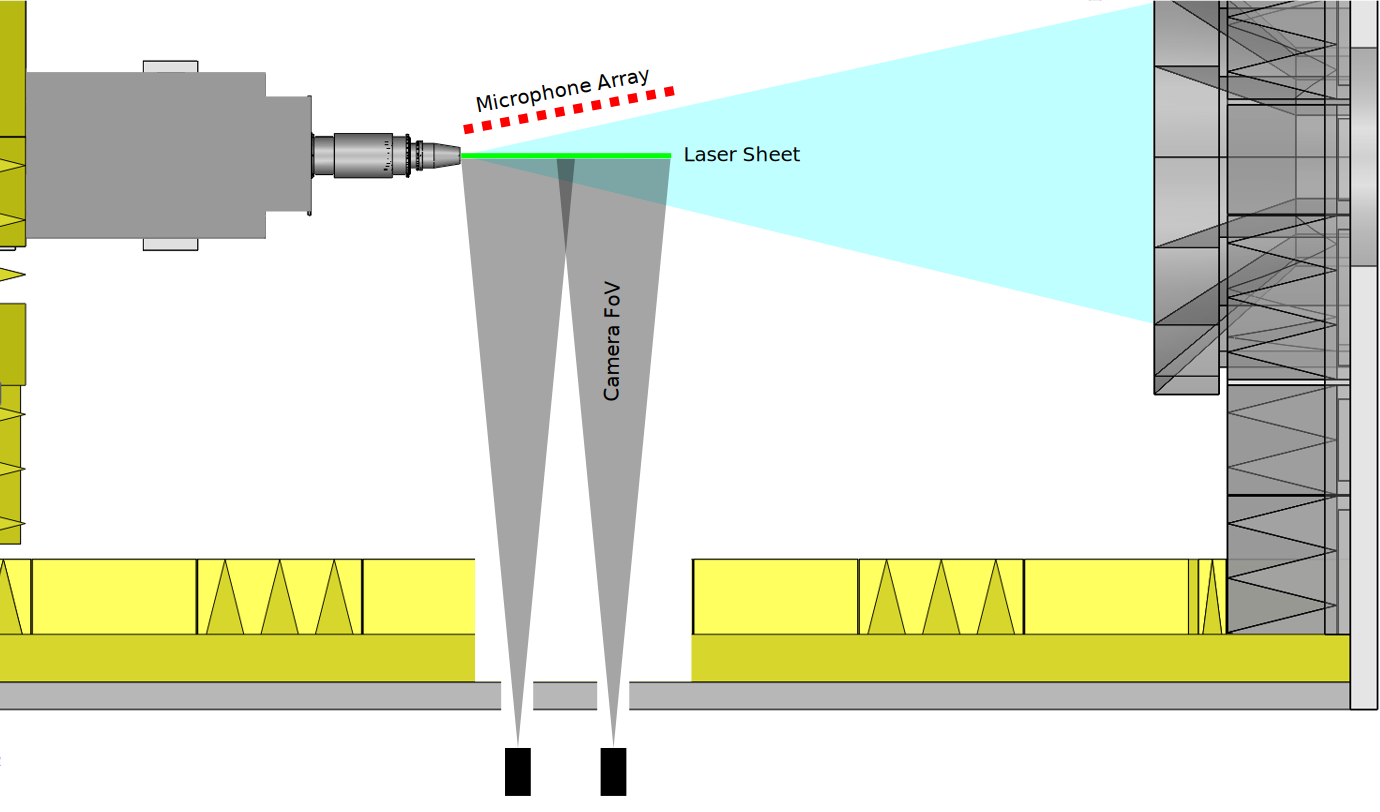
\includegraphics[width=6in]{Figures/ch2_piv_setup.png}
	\caption{Schematic of syncronized PIV and near-field pressure data acquisition setup.}
	\label{fig:piv_setup}
\end{figure}

The image groups were acquired in two modes: ensemble and phase-locked. 
When in phase-locked mode, a reference signal from the LAFPA control computer was used as an external trigger for LaVision's DaVis software; various filters were placed inline in order to damp the electromagnetic interference generated by the LAFPAs.
The reference signal was downsampled to roughly 10 Hz by the LAFPA control computer, and delayed appropriately in time to control the acquired actuation phase.
For this case, 300 image groups were acquired for an individual phase. 
In ensemble mode, image groups were acquired randomly in time at the system's maximum acquisition rate (5 Hz).
In this case, the PIV computer was set to output a reference signal which was used to trigger the acoustics data acquisition system.
The timing was set such that the PIV image acquisition would occur roughly in the center of a data block acquired by the acoustics system; the signal from a ThorLabs DET210 photoreceiver was also recorded in order to accurately identify the timing of the image acquisition in relation to the pressure time traces.
For this case, 1500 image groups were acquired for each case.

Instantaneous velocity vectors were computed using LaVision's DaVis software.
Multipass, FFT-based cross-correlations were used, with decreasing window size (64$\times$64 for the initial pass, and 32$\times$32 for the final three passes).
A 50\% overlap was used for the initial pass, and a 75\% overlap was used for all subsequent passes.
An Gaussian window (elliptic in the streamwise direction) was applied to the correlation windows.
The velocity fields were post-processed to remove spurious vectors, which were iteratively replaced if secondary correlation peaks were found, before the downstream and upstream images were combined.
No interpolation, smoothing, or denoising was performed in post-processing.

Due to the nature of the plasma actuators used in these experiments (pulsed DC), electromagnetic interference (EMI) and radio-frequency interference (RFI) were significant concerns during data acquisition.
Signal corruption could not only lead to excessively noisy data, but cause a mis-trigger event to occur between the laser, cameras, or microphones which would lead to garbage data.
Great pains were therefore taken in order to isolate, shield and filter the electrical systems.
A fiber-optic relay was designed and built in order to electrically isolate the plasma-generating equipment from the control computer (and ultimately the data acquisition systems).
The plasma-generating equipment was also enclosed in a grounded metal rackmount cart to reduce the emitted RFI.
Unfortunately, the building electrical grounds were also found to be corrupted by EMI, so additional filters were placed in stages along the trigger signal.
A BenchMaster 21M Kemo filter, set to low-pass mode with a cutoff frequency of 99 kHz, was used to filter the flashlamp and q-switch trigger signals going into the laser power supply and head.
Finally, between the LAFPA control computer and the PIV programmable timing unit input trigger a set of custom inductor-capacitor, resister-capacitor, and transient-voltage-suppressor filters were used. 